\documentclass[a4paper]{article}

%% Language and font encodings
\usepackage[english]{babel}
\usepackage[utf8x]{inputenc}
\usepackage[T1]{fontenc}

%% Sets page size and margins
\usepackage[a4paper,top=3cm,bottom=2cm,left=3cm,right=3cm,marginparwidth=1.75cm]{geometry}

%% Useful packages
\usepackage{amsmath}
\usepackage{graphicx}
\usepackage{mathtools}
\usepackage[colorinlistoftodos]{todonotes}
\usepackage[colorlinks=true, allcolors=blue]{hyperref}

\title{Training a Neural Network - A Numerical Example}
\author{Raphael B. Alampay}

\begin{document}
\maketitle

\begin{abstract}
Neural networks are models used to approximate a discriminative function for classification in a supervised learning fashion. You have a bunch of input in the form of $n$-dimensional numerical vectors that represent features of certain entities you'd like to teach the network to classify (example 1000 emails classified as spam and 1000 emails classified non-spam). This paper takes a look at a quantitative approach in training a neural network given actual numerical examples. This will allow the student/practitioner to understand the fundamentals of the training process namely feed forward and backpropagation. The paper is intended to be light in concept with specific examples for people getting into machine learning with neural networks.
\end{abstract}

\section{Introduction}
Neural networks are biologically inspired computational models that attempts to solve classification problems. It is composed on \textbf{neurons} which holds and processes values in the network. You can think of these values as signal strengths that aim to mimic how chemical reactions occur in the brain. The higher the value, the stronger the signal. In biology, neurons transmit and receive signals to and from other neurons by means of dendrites. These propagations are modelled in the neural network by means of weight values. Since a neuron may receive values from more than one neuron, it accounts all the weights connected to it before attempting to fire a signal thus simulating how we "react" to certain stimuli. Training the neural network roughly means looking for the optimal values for these weights based on what we already know in order for the model to properly "react" to a certain input.

\begin{figure}[!htb]
\centering
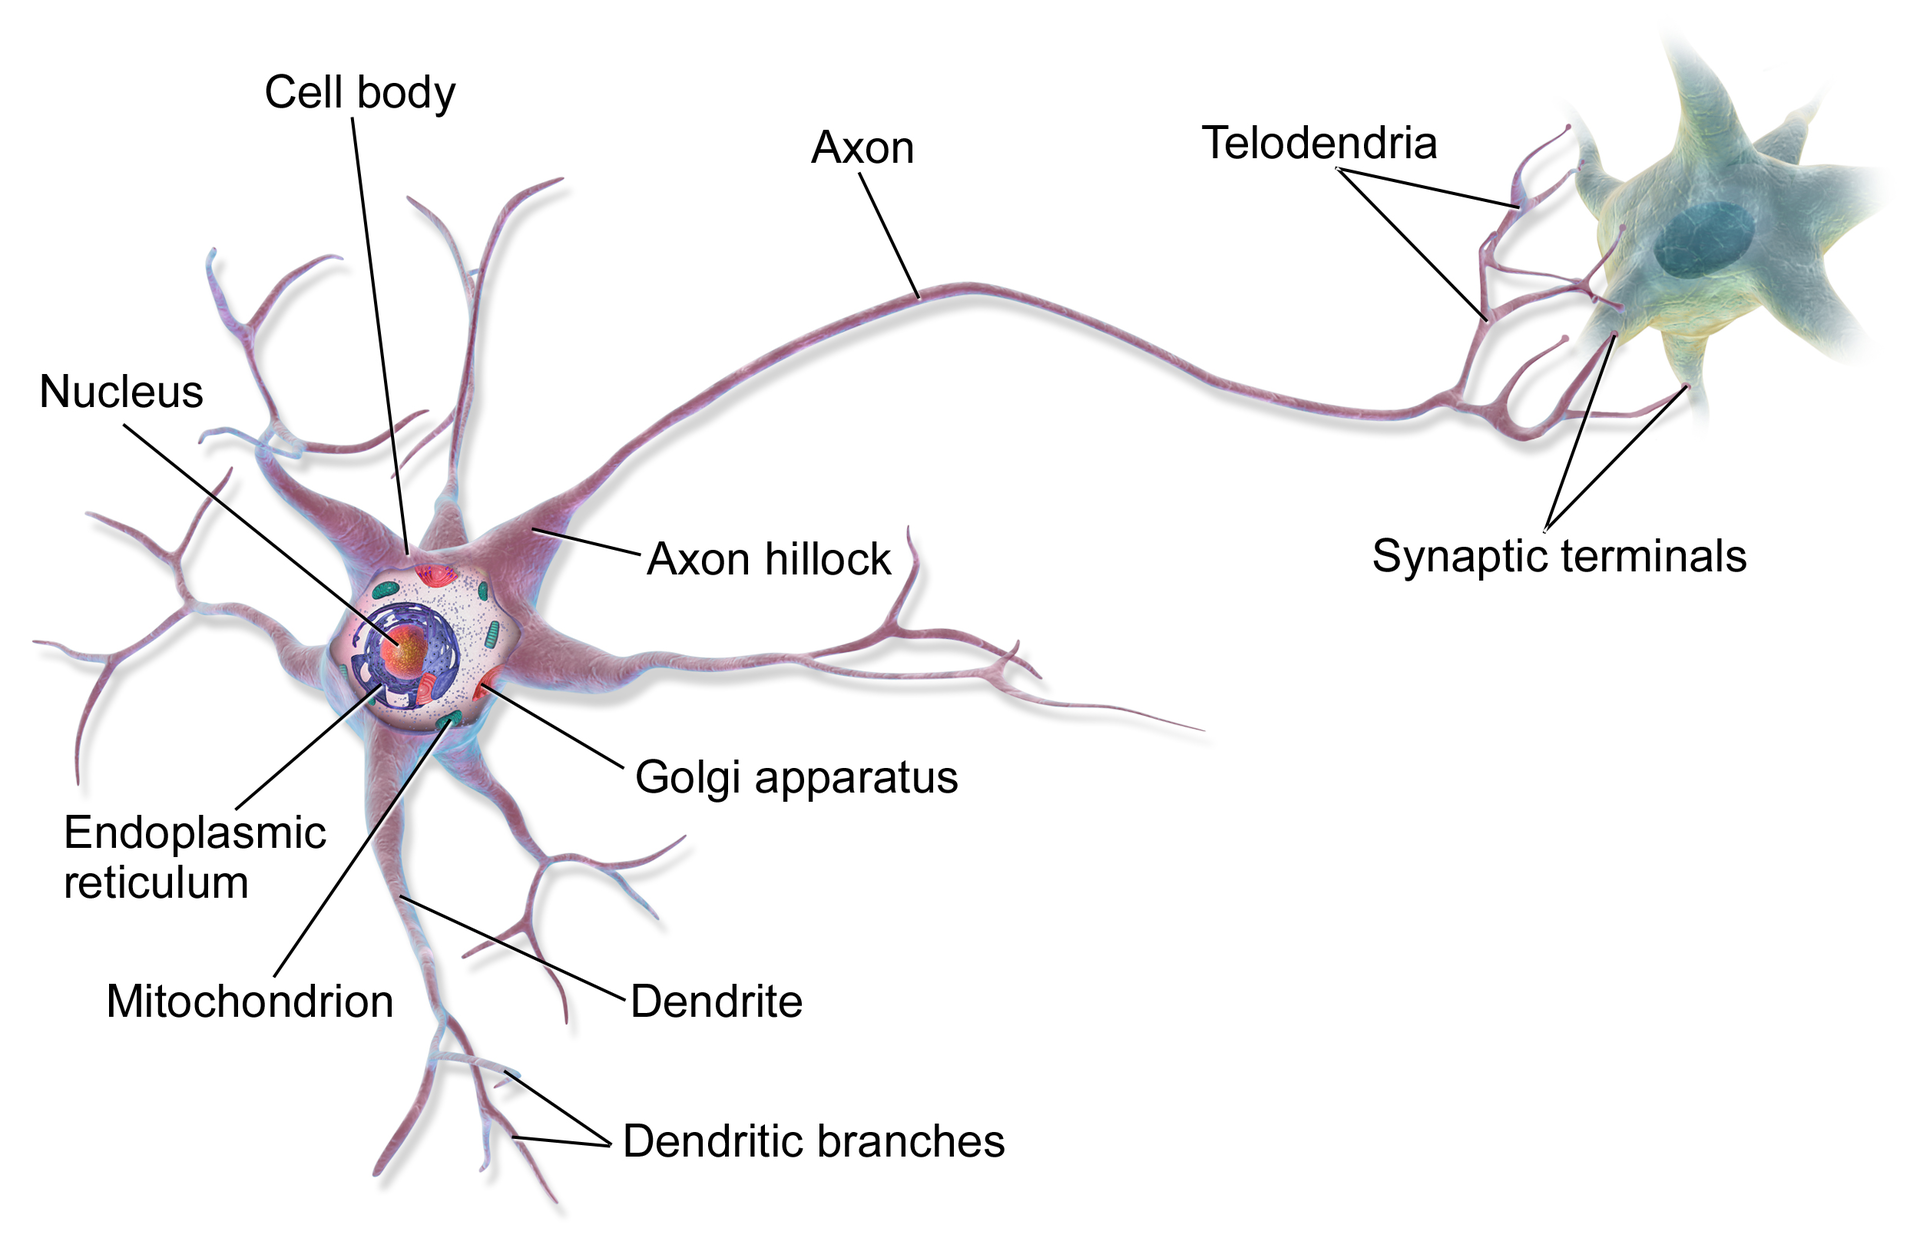
\includegraphics[width=0.5\textwidth]{neuron.png}
\caption{\label{fig:neuron}An example of a neuron taken from wikipedia.}
\end{figure}

There are typically 3 layers in a classical neural network - \textbf{input layer}, \textbf{hidden layer/s} and \textbf{output layer}. These layers are connected to one another via neurons' weights in an adjacent manner. This means that a layer can only be connected to at most two adjacent layers. The \textbf{input layer} will always be the leftmost layer, the \textbf{output layer} will always be the rightmost layer while everything in between will be \textbf{hidden layers}. The following example is an illustration of the classical neural network:

\begin{figure}[!htb]
\centering
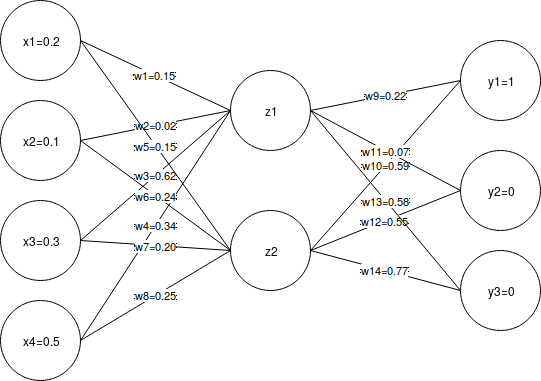
\includegraphics[width=0.5\textwidth]{neural_network.png}
\caption{\label{fig:neuron}A neural network with 4 neurons in the input layer, 2 for hidden and 3 for output}
\end{figure}

\subsection{Input Layer}
The input layer contains neurons that represent the input values or what the network initially receives from the real world. These values are features that represent a classification/label that we'd like to recognize. In the mathematical model $f(x) = y$, this would be the $x$ as an $n$-dimensional vector. For example, if we'd like to tell the neural network that we're looking at an image of a face represented by a matrix of pixel values, and suppose the size of the image is 32 x 32 pixels, the input layer would have a total of $1024$ neurons each one corresponding to a pixel value. We refer to this vector as a \textbf{feature vector}.

\subsection{Hidden Layer/s}
From the input layer, information is passed to a hidden layer which contains neurons that processes signals it receives from the its adjacent layer/s (either from the left or from the right). A neural network can have more than one hidden layer. Neurons in the hidden layer are often denoted as $z_{i}$ which we refer to as \textbf{latent variables}.

\subsection{Output Layer}
The output layer contains neurons that represent the output of the network or the result/reaction of the network after receiving and processing the input (from input layer to hidden layer then finally to the output layer). The easiest way to model neurons in the output layer is to treat each one (neuron) as a classification/label that the network is trying to recognize with a value ranging from $0$ to $1$. The closer the value to $1$ for an output neuron, the closer it is to thinking that it is that classification or label for a given input $x$. For example, let's say we're trying to learn how to diffirentiate cats from dogs from any other animal. The set of possible outputs (cat, dog or others) can be represented by:

\begin{equation}
  Y=\begin{bmatrix}
    y_{1} &   y_{2} & y_{3}
  \end{bmatrix}
\end{equation}

where $y_{1}$ represents the label cat, $y_{2}$ dog and $y_{3}$ others. A cat then for a neural network would look like $f(x) = \begin{bmatrix} 1 &   0 & 0 \end{bmatrix}$, a dog would be $f(x) = \begin{bmatrix} 0 &  1 & 0 \end{bmatrix}$ and finally any other animal $f(x) = \begin{bmatrix} 0 & 0 & 1 \end{bmatrix}$.

\section{Training}

To train a neural network means to optimize the set of weights (connections between neurons) in such a way that when we give it a feature vector representing a cat, the output should be close to $f(x) = \begin{bmatrix} 1 & 0 & 0 \end{bmatrix}$. In order to do this, at the beginning of training, the weights are randomly initialized. We then feed it a feature vector relating to cat and see what the $Y$ value is --- how close did the network get to the actual answer. This closeness value can be measured by a \textbf{loss function}. A higher value for this function means that the network yielded a higher error while smaller value means that the network is getting pretty close to recognizing what the input is. We will use this error/closeness value to adjust the weights accordingly. The first step in this entire training process is called \textbf{feed forward}. 

For the rest of the discussion, we will be referring to figure 2 as reference. Initially, the weights of the network will be as follows:

\begin{equation}
  W_{1}=
    \begin{bmatrix}
      0.15  & 0.14 \\
      0.02  & 0.24 \\
      0.62  & 0.20 \\
      0.34  & 0.25 \\
    \end{bmatrix}
\end{equation}

\begin{equation}
  W_{2}=
    \begin{bmatrix}
      0.22 & 0.07 & 0.58 \\
      0.59 & 0.55 & 0.77
    \end{bmatrix}
\end{equation}


\subsection{Feed Forward}
The feed forward process can be thought of the movement of information from the input layer in the form of the feature vector's values to the first hidden layer and finally making the guess (classification) in the output layer. Given two consecutive layers, information is passed from the left layer to the right layer by performing a matrix multiplication operation between the left layer's neurons and the weight matrix between the left and right layer. The resulting matrix should have the same size as the neurons in the right layer (1 row with $n$ columns where $n$ is the size of the neurons in the right layer). Let's take the following illustration:

We're trying to solve for the values of $Z$ by matrix multiplying $X$ with $W_{1}$. The result will then be passed to an activation function such as the \textbf{sigmoid function} given by:

\begin{equation}
  a(x) = 1 / (1 + e^{-x})
\end{equation}

Mathematically, we can then represent information flow from $X$ to $Z$:

\begin{equation}
  Z=a((X)(W_{1}))
\end{equation}

Numerically we have the following:

\begin{equation}
  Z=\begin{bmatrix}
      0.2 & 0.1 & 0.3 & 0.5
    \end{bmatrix}
    \begin{bmatrix}
      0.15  & 0.14 \\
      0.02  & 0.24 \\
      0.62  & 0.20 \\
      0.34  & 0.25 \\
    \end{bmatrix}
\end{equation}

\begin{equation}
  Z=\begin{bmatrix}
      0.388 & 0.237
    \end{bmatrix}
\end{equation}
\begin{equation}
  Z=a(\begin{bmatrix}
      0.388 & 0.237
    \end{bmatrix})
\end{equation}
\begin{equation}
  Z=\begin{bmatrix}
      0.5958 & 0.5590
    \end{bmatrix}
\end{equation}

Using the same approach, we feed forward $Z$'s values towards $Y$ by matrix multiplying it with $W_{2}$. 

Mathematically:

\begin{equation}
  Y=a((Z_{1})(W_{2}))
\end{equation}

Numerically:

\begin{equation}
  Y=\begin{bmatrix}
      0.5958 & 0.5590
    \end{bmatrix}
    \begin{bmatrix}
      0.22 & 0.07 & 0.58 \\
      0.59 & 0.55 & 0.77
    \end{bmatrix}
\end{equation}

\begin{equation}
  Y=\begin{bmatrix}
      0.4609 & 0.3491 & 0.7760
    \end{bmatrix}
\end{equation}

\begin{equation}
  Y=a(\begin{bmatrix}
      0.4609 & 0.3491 & 0.7760
    \end{bmatrix})
\end{equation}

\begin{equation}
  Y=\begin{bmatrix}
      0.6132 & 0.5864 & 0.6848
    \end{bmatrix}
\end{equation}

\subsection{Loss Function}

The loss function determines how far (or close) the guess of the network ($Y$) to the actual classification value ($\widehat{Y}$). Remember that we want to teach the network how to recognize a certain classification by adjusting the its weights. The amount of adjustment we do will largely depend on the value given by the \textbf{loss function}. For this paper, we will be using a very simple loss function:

\begin{equation}
  E(Y, \widehat{Y})=\sum_{i}^{n} {(Y_{i}-\widehat{Y_{i}})^2}
\end{equation}

In the case of our example, $\widehat{Y}=\begin{bmatrix}1 & 0 & 0\end{bmatrix}$, the value of our loss function will be computed as:

\begin{equation}
  E(Y, \widehat{Y})=\sum_{i}^{n}(\begin{bmatrix}0.6132 & 0.5864 & 0.6848\end{bmatrix} - \begin{bmatrix}1 & 0 & 0\end{bmatrix})^2
\end{equation}

Decomposing it we have:

\begin{equation}
  e_{1} = (0.6132 - 1)^2
\end{equation}
\begin{equation}
  e_{2} = (0.5864 - 0)^2
\end{equation}
\begin{equation}
  e_{3} = (0.6848 - 0)^2
\end{equation}

\begin{equation}
  E(Y, \widehat{Y})=e_{1} + e_{2} + e_{3}
\end{equation}

\begin{equation}
  E(Y, \widehat{Y})=0.1496 + 0.3439 + 0.4690
\end{equation}
\begin{equation}
  E(Y, \widehat{Y})=0.9624
\end{equation}

\subsection{Back Propagation}

Once we get the error value from the loss function, we can use this value to determine how much change we would apply to the weights to minimize this error value. This is done by a process called back propagation which takes the individual error values and cascades it from the output layer to the input layer seeing how much damage the weight values contributed to the overall error. Integral to this process is to solve for \textbf{gradients}. These gradients are approximation of derivatives. As with derivatives, gradient values dictate the direction of the error function of the network. If we know these values, we can roughly determine how to adjust our weights to minimize the error. To simplify things, since weight values drive the error value, we'd like to determine the gradient values for each neuron (since weights are attached to neurons) starting from the output layer (thus backward propagation) to give us the \textbf{delta weights} or how much magnitude should we adjust the original weights to lower the error. Numerically, this means that the size of our gradient vector will be the same size of neurons in a given layer.

For a more specific example, we'll break down this process into two major operations. The first part will perform back propagation starting from the output to the last hidden layer. And the second part will be from the last hidden layer down to the input layer. Similar to feed forward, we will be computing values with 3 inputs -- 2 layers and the weight matrix in between them. For each pair of layers, the gradient values to be computed for the right layer.

\subsubsection{BP from Output to Last Hidden Layer}
To start off, we compute the gradients for the right layer in this part of BP which in this case is the output layer ($Y$).

\subsubsection{BP from Last Hidden to Input Layer}

\section{Some examples to get started}

\[ \left( \begin{array}{cc}
1 & 0 \\
0 & 1
\end{array} \right)^{T}
%
=
\left( \begin{array}{cc}
1 & 0 \\
0 & 1
\end{array} \right)
\]

\subsection{How to add Comments}

Comments can be added to your project by clicking on the comment icon in the toolbar above. % * <john.hammersley@gmail.com> 2016-07-03T09:54:16.211Z:
%
% Here's an example comment!
%
To reply to a comment, simply click the reply button in the lower right corner of the comment, and you can close them when you're done.

Comments can also be added to the margins of the compiled PDF using the todo command\todo{Here's a comment in the margin!}, as shown in the example on the right. You can also add inline comments:

\todo[inline, color=green!40]{This is an inline comment.}

\subsection{How to write Mathematics}

\LaTeX{} is great at typesetting mathematics. Let $X_1, X_2, \ldots, X_n$ be a sequence of independent and identically distributed random variables with $\text{E}[X_i] = \mu$ and $\text{Var}[X_i] = \sigma^2 < \infty$, and let
\[S_n = \frac{X_1 + X_2 + \cdots + X_n}{n}
      = \frac{1}{n}\sum_{i}^{n} X_i\]
denote their mean. Then as $n$ approaches infinity, the random variables $\sqrt{n}(S_n - \mu)$ converge in distribution to a normal $\mathcal{N}(0, \sigma^2)$.


\subsection{How to create Sections and Subsections}

Use section and subsections to organize your document. Simply use the section and subsection buttons in the toolbar to create them, and we'll handle all the formatting and numbering automatically.

\subsection{How to add Lists}

You can make lists with automatic numbering \dots

\begin{enumerate}
\item Like this,
\item and like this.
\end{enumerate}
\dots or bullet points \dots
\begin{itemize}
\item Like this,
\item and like this.
\end{itemize}

\subsection{How to add Citations and a References List}

You can upload a \verb|.bib| file containing your BibTeX entries, created with JabRef; or import your \href{https://www.overleaf.com/blog/184}{Mendeley}, CiteULike or Zotero library as a \verb|.bib| file. You can then cite entries from it, like this: \cite{greenwade93}. Just remember to specify a bibliography style, as well as the filename of the \verb|.bib|.

You can find a \href{https://www.overleaf.com/help/97-how-to-include-a-bibliography-using-bibtex}{video tutorial here} to learn more about BibTeX.

We hope you find Overleaf useful, and please let us know if you have any feedback using the help menu above --- or use the contact form at \url{https://www.overleaf.com/contact}!

\bibliographystyle{alpha}
\bibliography{sample}

\end{document}
